\documentclass[14pt]{extbook}
\usepackage{multicol, enumerate, enumitem, hyperref, color, soul, setspace, parskip, fancyhdr} %General Packages
\usepackage{amssymb, amsthm, amsmath, latexsym, units, mathtools} %Math Packages
\everymath{\displaystyle} %All math in Display Style
% Packages with additional options
\usepackage[headsep=0.5cm,headheight=12pt, left=1 in,right= 1 in,top= 1 in,bottom= 1 in]{geometry}
\usepackage[usenames,dvipsnames]{xcolor}
\usepackage{dashrule}  % Package to use the command below to create lines between items
\newcommand{\litem}[1]{\item#1\hspace*{-1cm}\rule{\textwidth}{0.4pt}}
\pagestyle{fancy}
\lhead{Progress Quiz 10}
\chead{}
\rhead{Version ALL}
\lfoot{5170-5105}
\cfoot{}
\rfoot{Summer C 2021}
\begin{document}

\begin{enumerate}
\litem{
Choose the equation of the function graphed below.
\begin{center}
    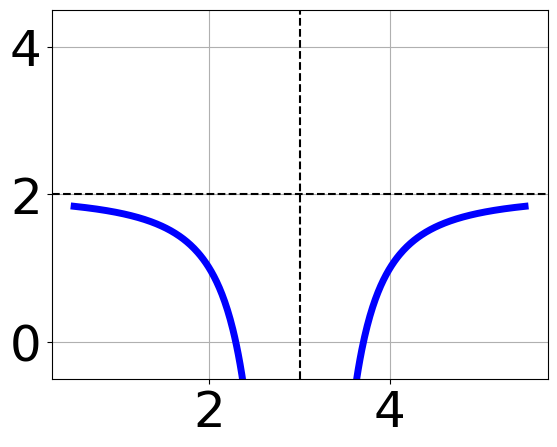
\includegraphics[width=0.5\textwidth]{../Figures/rationalGraphToEquationCopyA.png}
\end{center}
\begin{enumerate}[label=\Alph*.]
\item \( f(x) = \frac{1}{x + 3} + 2 \)
\item \( f(x) = \frac{-1}{(x - 3)^2} + 2 \)
\item \( f(x) = \frac{-1}{x - 3} + 2 \)
\item \( f(x) = \frac{1}{(x + 3)^2} + 2 \)
\item \( \text{None of the above} \)

\end{enumerate} }
\litem{
Solve the rational equation below. Then, choose the interval(s) that the solution(s) belongs to.\[ \frac{-88}{99x + 22} + 1 = \frac{-88}{99x + 22} \]\begin{enumerate}[label=\Alph*.]
\item \( x_1 \in [-1.1, -0.1] \text{ and } x_2 \in [-0.34,-0.04] \)
\item \( x_1 \in [-1.1, -0.1] \text{ and } x_2 \in [0.17,0.28] \)
\item \( x \in [0.1,1.8] \)
\item \( x \in [-0.22,2.78] \)
\item \( \text{All solutions lead to invalid or complex values in the equation.} \)

\end{enumerate} }
\litem{
Determine the domain of the function below.\[ f(x) = \frac{6}{12x^{2} -12} \]\begin{enumerate}[label=\Alph*.]
\item \( \text{All Real numbers.} \)
\item \( \text{All Real numbers except } x = a, \text{ where } a \in [-17.4, -14.6] \)
\item \( \text{All Real numbers except } x = a \text{ and } x = b, \text{ where } a \in [-17.4, -14.6] \text{ and } b \in [8.4, 9.8] \)
\item \( \text{All Real numbers except } x = a, \text{ where } a \in [-3.6, -0.6] \)
\item \( \text{All Real numbers except } x = a \text{ and } x = b, \text{ where } a \in [-3.6, -0.6] \text{ and } b \in [0.1, 2.5] \)

\end{enumerate} }
\litem{
Choose the graph of the equation below.\[ f(x) = \frac{1}{(x - 1)^2} - 2 \]\begin{enumerate}[label=\Alph*.]
\begin{multicols}{2}\item 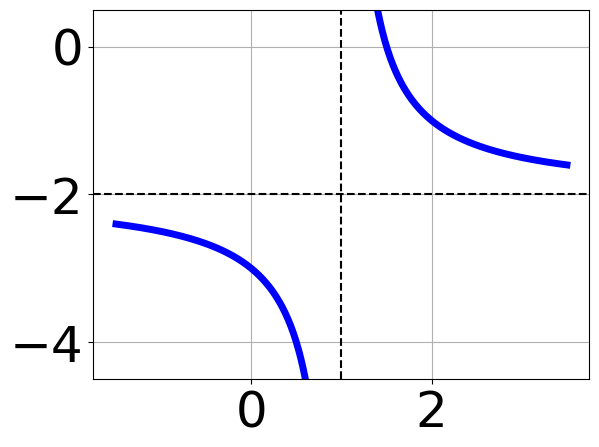
\includegraphics[width = 0.3\textwidth]{../Figures/rationalEquationToGraphCopyAA.png}\item 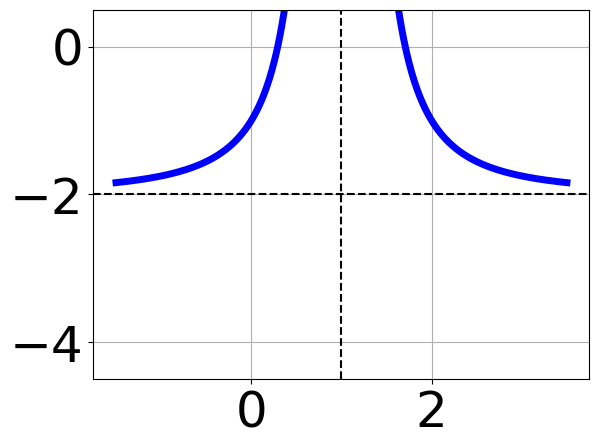
\includegraphics[width = 0.3\textwidth]{../Figures/rationalEquationToGraphCopyBA.png}\item 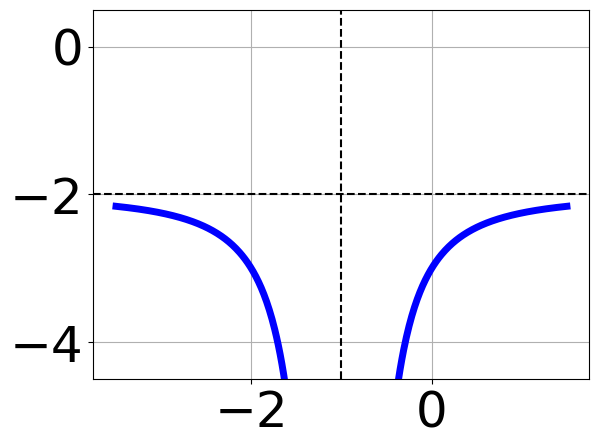
\includegraphics[width = 0.3\textwidth]{../Figures/rationalEquationToGraphCopyCA.png}\item 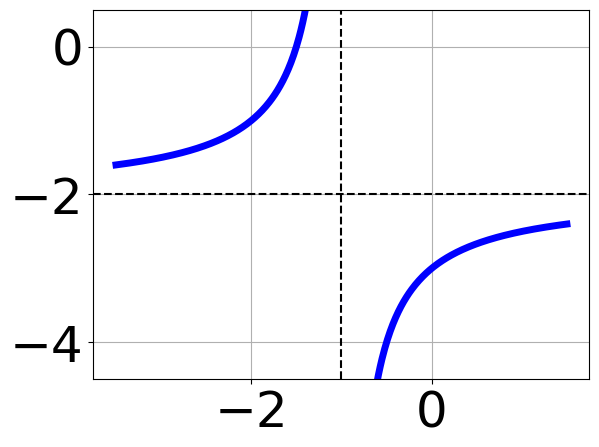
\includegraphics[width = 0.3\textwidth]{../Figures/rationalEquationToGraphCopyDA.png}\end{multicols}\item None of the above.
\end{enumerate} }
\litem{
Solve the rational equation below. Then, choose the interval(s) that the solution(s) belongs to.\[ \frac{4x}{-2x + 3} + \frac{-4x^{2}}{-8x^{2} +4 x + 12} = \frac{7}{4x + 4} \]\begin{enumerate}[label=\Alph*.]
\item \( x \in [-1.33,0.28] \)
\item \( x_1 \in [-0.84, 2.52] \text{ and } x_2 \in [-0.5,4.5] \)
\item \( x_1 \in [-0.84, 2.52] \text{ and } x_2 \in [-11.07,0.93] \)
\item \( \text{All solutions lead to invalid or complex values in the equation.} \)
\item \( x \in [-3.83,-2.24] \)

\end{enumerate} }
\litem{
Choose the equation of the function graphed below.
\begin{center}
    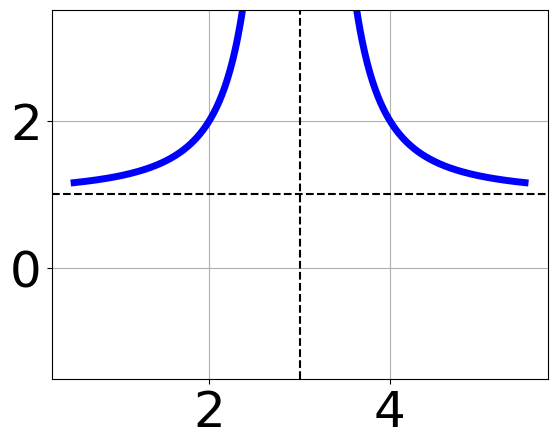
\includegraphics[width=0.5\textwidth]{../Figures/rationalGraphToEquationA.png}
\end{center}
\begin{enumerate}[label=\Alph*.]
\item \( f(x) = \frac{-1}{x - 3} + 8 \)
\item \( f(x) = \frac{-1}{(x - 3)^2} + 8 \)
\item \( f(x) = \frac{1}{(x + 3)^2} + 8 \)
\item \( f(x) = \frac{1}{x + 3} + 8 \)
\item \( \text{None of the above} \)

\end{enumerate} }
\litem{
Determine the domain of the function below.\[ f(x) = \frac{6}{9x^{2} -27 x + 18} \]\begin{enumerate}[label=\Alph*.]
\item \( \text{All Real numbers.} \)
\item \( \text{All Real numbers except } x = a, \text{ where } a \in [8.93, 9.88] \)
\item \( \text{All Real numbers except } x = a \text{ and } x = b, \text{ where } a \in [0.73, 1.14] \text{ and } b \in [1.29, 2.13] \)
\item \( \text{All Real numbers except } x = a, \text{ where } a \in [0.73, 1.14] \)
\item \( \text{All Real numbers except } x = a \text{ and } x = b, \text{ where } a \in [8.93, 9.88] \text{ and } b \in [17.21, 18.34] \)

\end{enumerate} }
\litem{
Choose the graph of the equation below.\[ f(x) = \frac{-1}{x - 3} - 2 \]\begin{enumerate}[label=\Alph*.]
\begin{multicols}{2}\item 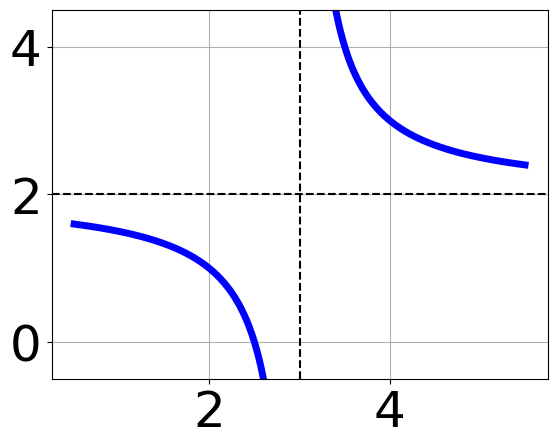
\includegraphics[width = 0.3\textwidth]{../Figures/rationalEquationToGraphAA.png}\item 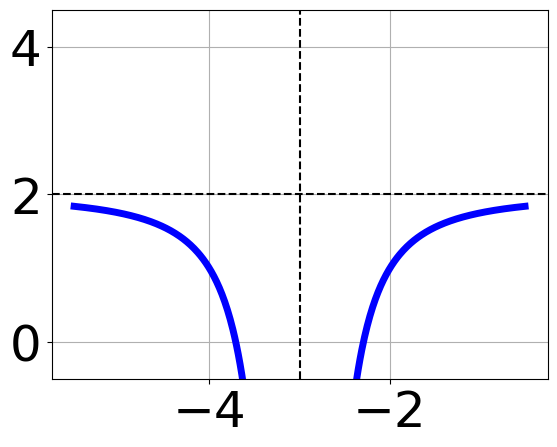
\includegraphics[width = 0.3\textwidth]{../Figures/rationalEquationToGraphBA.png}\item 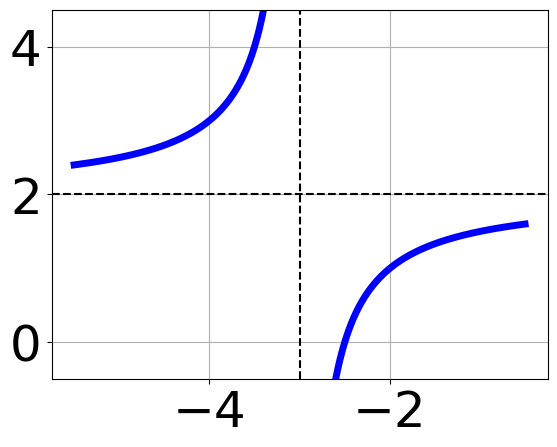
\includegraphics[width = 0.3\textwidth]{../Figures/rationalEquationToGraphCA.png}\item 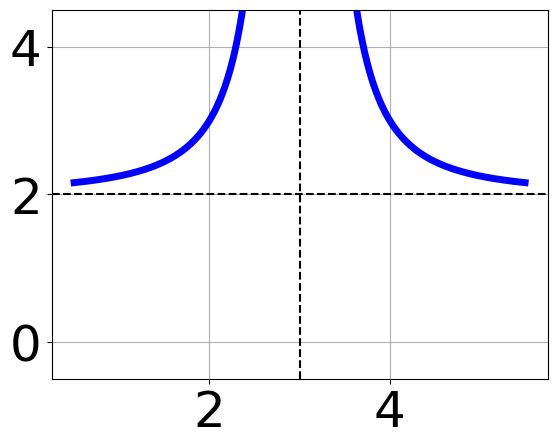
\includegraphics[width = 0.3\textwidth]{../Figures/rationalEquationToGraphDA.png}\end{multicols}\item None of the above.
\end{enumerate} }
\litem{
Solve the rational equation below. Then, choose the interval(s) that the solution(s) belongs to.\[ \frac{7x}{6x + 6} + \frac{-4x^{2}}{36x^{2} +60 x + 24} = \frac{-7}{6x + 4} \]\begin{enumerate}[label=\Alph*.]
\item \( x_1 \in [-1.14, -0.86] \text{ and } x_2 \in [-0.7,-0.47] \)
\item \( \text{All solutions lead to invalid or complex values in the equation.} \)
\item \( x_1 \in [-1.47, -1.1] \text{ and } x_2 \in [-0.59,-0.06] \)
\item \( x \in [-1.14,-0.86] \)
\item \( x \in [-0.76,-0.61] \)

\end{enumerate} }
\litem{
Solve the rational equation below. Then, choose the interval(s) that the solution(s) belongs to.\[ \frac{20}{-40x + 20} + 1 = \frac{20}{-40x + 20} \]\begin{enumerate}[label=\Alph*.]
\item \( x \in [0.5,2.5] \)
\item \( x_1 \in [-1, 0.1] \text{ and } x_2 \in [-0.5,2.5] \)
\item \( x \in [-1,0.1] \)
\item \( x_1 \in [0, 1.1] \text{ and } x_2 \in [-0.5,2.5] \)
\item \( \text{All solutions lead to invalid or complex values in the equation.} \)

\end{enumerate} }
\litem{
Choose the equation of the function graphed below.
\begin{center}
    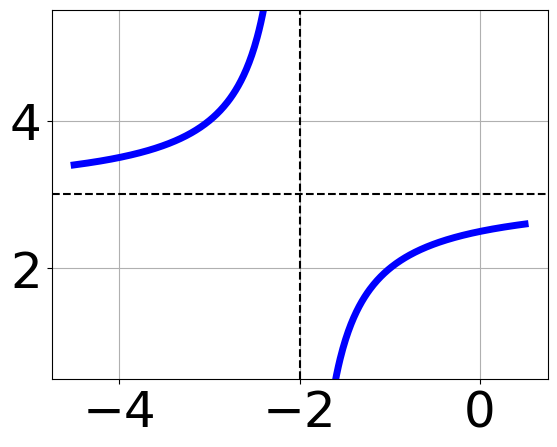
\includegraphics[width=0.5\textwidth]{../Figures/rationalGraphToEquationCopyB.png}
\end{center}
\begin{enumerate}[label=\Alph*.]
\item \( f(x) = \frac{-1}{x + 2} + 3 \)
\item \( f(x) = \frac{1}{(x - 2)^2} + 3 \)
\item \( f(x) = \frac{-1}{(x + 2)^2} + 3 \)
\item \( f(x) = \frac{1}{x - 2} + 3 \)
\item \( \text{None of the above} \)

\end{enumerate} }
\litem{
Solve the rational equation below. Then, choose the interval(s) that the solution(s) belongs to.\[ \frac{-84}{84x + 36} + 1 = \frac{-84}{84x + 36} \]\begin{enumerate}[label=\Alph*.]
\item \( x \in [-1.43,0.57] \)
\item \( x \in [0,1.3] \)
\item \( x_1 \in [-0.7, 0.2] \text{ and } x_2 \in [-0.4,1.7] \)
\item \( x_1 \in [-0.7, 0.2] \text{ and } x_2 \in [-0.9,-0.2] \)
\item \( \text{All solutions lead to invalid or complex values in the equation.} \)

\end{enumerate} }
\litem{
Determine the domain of the function below.\[ f(x) = \frac{6}{25x^{2} +45 x + 18} \]\begin{enumerate}[label=\Alph*.]
\item \( \text{All Real numbers except } x = a \text{ and } x = b, \text{ where } a \in [-2.1, -0.7] \text{ and } b \in [-0.9, -0.2] \)
\item \( \text{All Real numbers except } x = a, \text{ where } a \in [-30.6, -29.5] \)
\item \( \text{All Real numbers except } x = a \text{ and } x = b, \text{ where } a \in [-30.6, -29.5] \text{ and } b \in [-15.9, -14.6] \)
\item \( \text{All Real numbers.} \)
\item \( \text{All Real numbers except } x = a, \text{ where } a \in [-2.1, -0.7] \)

\end{enumerate} }
\litem{
Choose the graph of the equation below.\[ f(x) = \frac{1}{(x + 3)^2} - 1 \]\begin{enumerate}[label=\Alph*.]
\begin{multicols}{2}\item 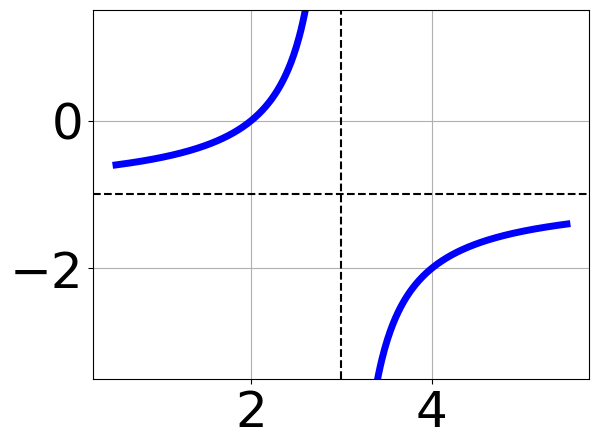
\includegraphics[width = 0.3\textwidth]{../Figures/rationalEquationToGraphCopyAB.png}\item 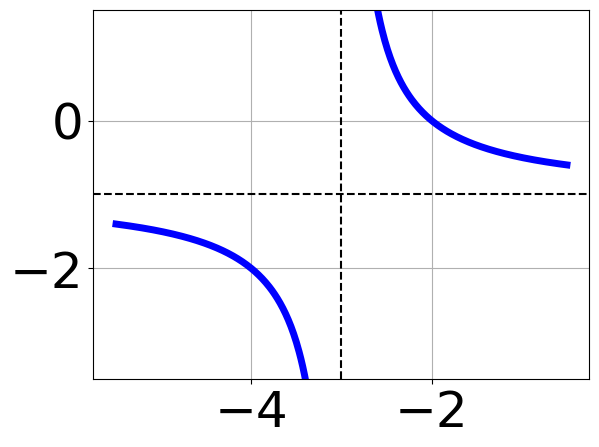
\includegraphics[width = 0.3\textwidth]{../Figures/rationalEquationToGraphCopyBB.png}\item 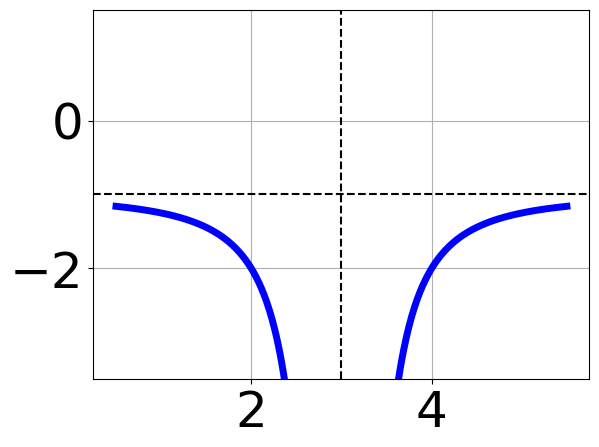
\includegraphics[width = 0.3\textwidth]{../Figures/rationalEquationToGraphCopyCB.png}\item 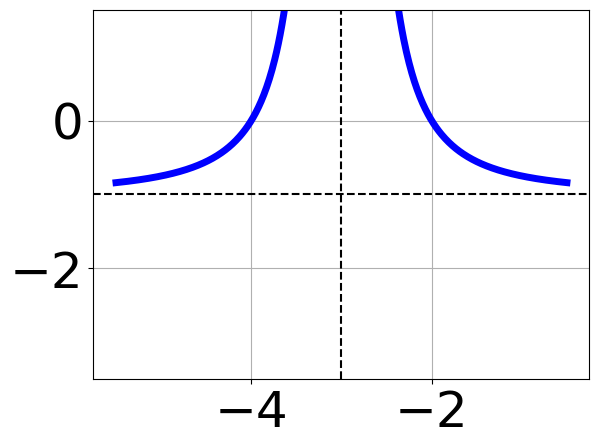
\includegraphics[width = 0.3\textwidth]{../Figures/rationalEquationToGraphCopyDB.png}\end{multicols}\item None of the above.
\end{enumerate} }
\litem{
Solve the rational equation below. Then, choose the interval(s) that the solution(s) belongs to.\[ \frac{-6x}{-7x -5} + \frac{-3x^{2}}{-14x^{2} -38 x -20} = \frac{-5}{2x + 4} \]\begin{enumerate}[label=\Alph*.]
\item \( \text{All solutions lead to invalid or complex values in the equation.} \)
\item \( x_1 \in [-3.93, -2.1] \text{ and } x_2 \in [-1.07,-0.51] \)
\item \( x \in [-2.81,-0.99] \)
\item \( x_1 \in [-3.93, -2.1] \text{ and } x_2 \in [-0.69,-0.27] \)
\item \( x \in [-0.99,0.12] \)

\end{enumerate} }
\litem{
Choose the equation of the function graphed below.
\begin{center}
    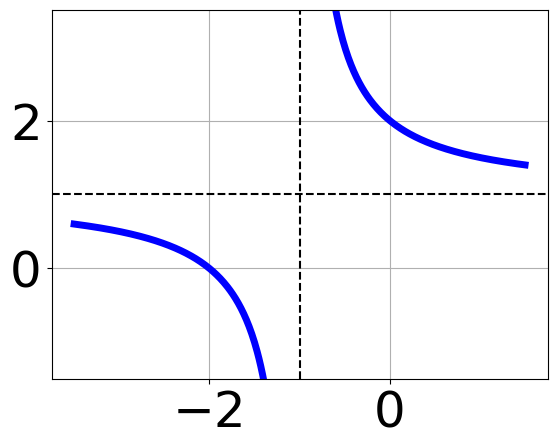
\includegraphics[width=0.5\textwidth]{../Figures/rationalGraphToEquationB.png}
\end{center}
\begin{enumerate}[label=\Alph*.]
\item \( f(x) = \frac{-1}{x - 1} + 1 \)
\item \( f(x) = \frac{1}{x + 1} + 1 \)
\item \( f(x) = \frac{-1}{(x - 1)^2} + 1 \)
\item \( f(x) = \frac{1}{(x + 1)^2} + 1 \)
\item \( \text{None of the above} \)

\end{enumerate} }
\litem{
Determine the domain of the function below.\[ f(x) = \frac{4}{15x^{2} +24 x + 9} \]\begin{enumerate}[label=\Alph*.]
\item \( \text{All Real numbers.} \)
\item \( \text{All Real numbers except } x = a, \text{ where } a \in [-15.49, -14.95] \)
\item \( \text{All Real numbers except } x = a \text{ and } x = b, \text{ where } a \in [-15.49, -14.95] \text{ and } b \in [-9.13, -8.74] \)
\item \( \text{All Real numbers except } x = a \text{ and } x = b, \text{ where } a \in [-1.44, -0.83] \text{ and } b \in [-0.78, -0.34] \)
\item \( \text{All Real numbers except } x = a, \text{ where } a \in [-1.44, -0.83] \)

\end{enumerate} }
\litem{
Choose the graph of the equation below.\[ f(x) = \frac{1}{(x + 3)^2} + 3 \]\begin{enumerate}[label=\Alph*.]
\begin{multicols}{2}\item 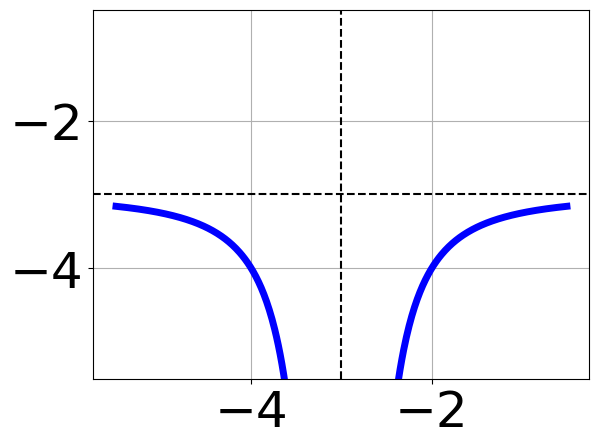
\includegraphics[width = 0.3\textwidth]{../Figures/rationalEquationToGraphAB.png}\item 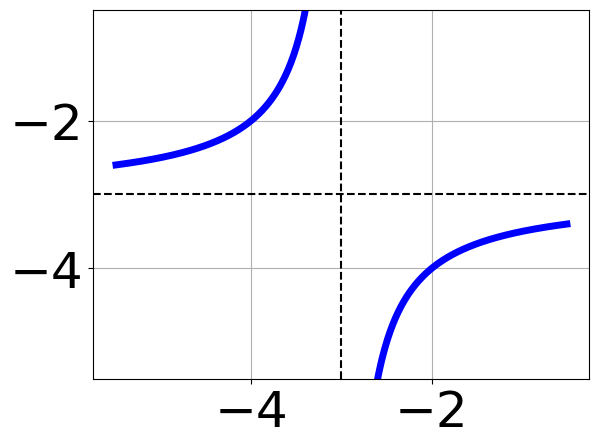
\includegraphics[width = 0.3\textwidth]{../Figures/rationalEquationToGraphBB.png}\item 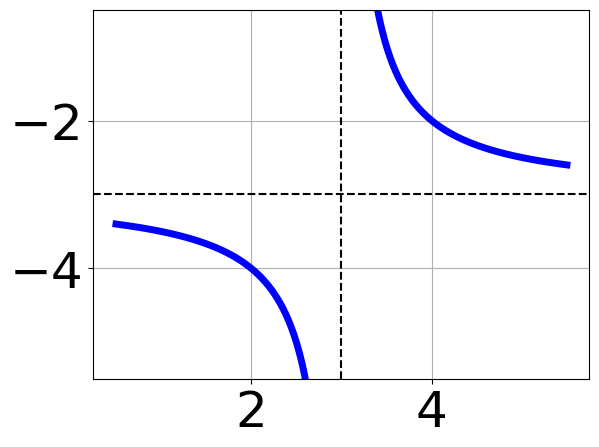
\includegraphics[width = 0.3\textwidth]{../Figures/rationalEquationToGraphCB.png}\item 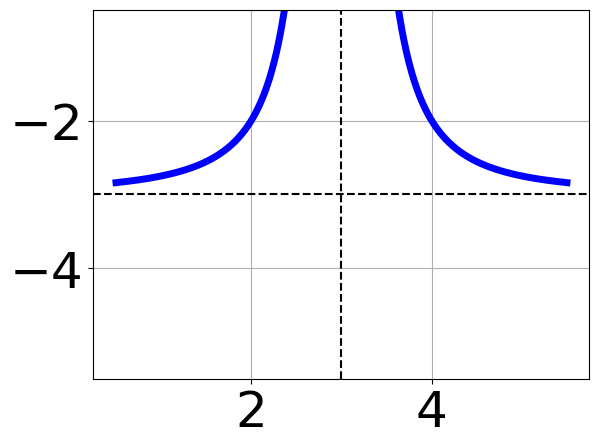
\includegraphics[width = 0.3\textwidth]{../Figures/rationalEquationToGraphDB.png}\end{multicols}\item None of the above.
\end{enumerate} }
\litem{
Solve the rational equation below. Then, choose the interval(s) that the solution(s) belongs to.\[ \frac{-5x}{4x + 3} + \frac{-2x^{2}}{-12x^{2} +19 x + 21} = \frac{-7}{-3x + 7} \]\begin{enumerate}[label=\Alph*.]
\item \( \text{All solutions lead to invalid or complex values in the equation.} \)
\item \( x \in [2.32,2.42] \)
\item \( x \in [-0.88,-0.65] \)
\item \( x_1 \in [-0.97, -0.81] \text{ and } x_2 \in [0.47,1.31] \)
\item \( x_1 \in [-0.88, -0.65] \text{ and } x_2 \in [2.07,3.03] \)

\end{enumerate} }
\litem{
Solve the rational equation below. Then, choose the interval(s) that the solution(s) belongs to.\[ \frac{-24}{60x -24} + 1 = \frac{-24}{60x -24} \]\begin{enumerate}[label=\Alph*.]
\item \( x_1 \in [-0.5, -0.2] \text{ and } x_2 \in [0.4,2.4] \)
\item \( x_1 \in [0.3, 0.8] \text{ and } x_2 \in [0.4,2.4] \)
\item \( x \in [0.4,1.4] \)
\item \( \text{All solutions lead to invalid or complex values in the equation.} \)
\item \( x \in [-0.5,-0.2] \)

\end{enumerate} }
\litem{
Choose the equation of the function graphed below.
\begin{center}
    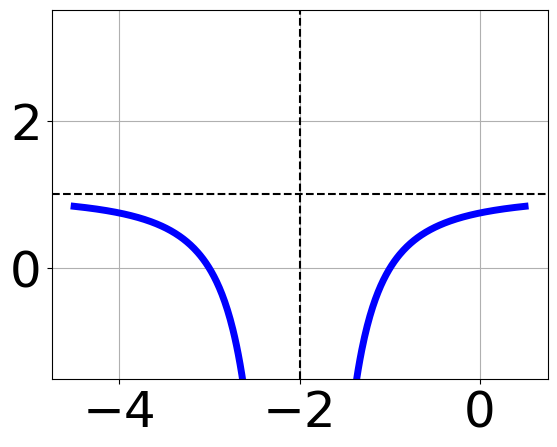
\includegraphics[width=0.5\textwidth]{../Figures/rationalGraphToEquationCopyC.png}
\end{center}
\begin{enumerate}[label=\Alph*.]
\item \( f(x) = \frac{1}{(x - 2)^2} + 1 \)
\item \( f(x) = \frac{-1}{x + 2} + 1 \)
\item \( f(x) = \frac{-1}{(x + 2)^2} + 1 \)
\item \( f(x) = \frac{1}{x - 2} + 1 \)
\item \( \text{None of the above} \)

\end{enumerate} }
\litem{
Solve the rational equation below. Then, choose the interval(s) that the solution(s) belongs to.\[ \frac{8}{-4x + 2} + 2 = \frac{-3}{-32x + 16} \]\begin{enumerate}[label=\Alph*.]
\item \( x_1 \in [1, 2.3] \text{ and } x_2 \in [1.83,2.12] \)
\item \( \text{All solutions lead to invalid or complex values in the equation.} \)
\item \( x_1 \in [0.5, 1.2] \text{ and } x_2 \in [1.49,1.64] \)
\item \( x \in [1.55,2.55] \)
\item \( x \in [0.5,1.2] \)

\end{enumerate} }
\litem{
Determine the domain of the function below.\[ f(x) = \frac{3}{30x^{2} +10 x -20} \]\begin{enumerate}[label=\Alph*.]
\item \( \text{All Real numbers except } x = a \text{ and } x = b, \text{ where } a \in [-1.3, 0.2] \text{ and } b \in [0.2, 1.4] \)
\item \( \text{All Real numbers except } x = a, \text{ where } a \in [-1.3, 0.2] \)
\item \( \text{All Real numbers except } x = a, \text{ where } a \in [-25.6, -24.6] \)
\item \( \text{All Real numbers except } x = a \text{ and } x = b, \text{ where } a \in [-25.6, -24.6] \text{ and } b \in [22.6, 25.6] \)
\item \( \text{All Real numbers.} \)

\end{enumerate} }
\litem{
Choose the graph of the equation below.\[ f(x) = \frac{-1}{x - 3} + 1 \]\begin{enumerate}[label=\Alph*.]
\begin{multicols}{2}\item 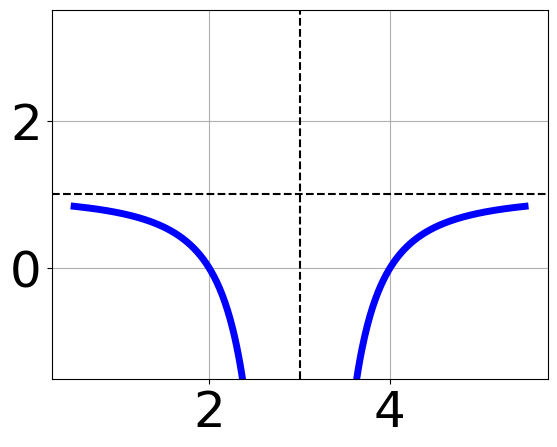
\includegraphics[width = 0.3\textwidth]{../Figures/rationalEquationToGraphCopyAC.png}\item 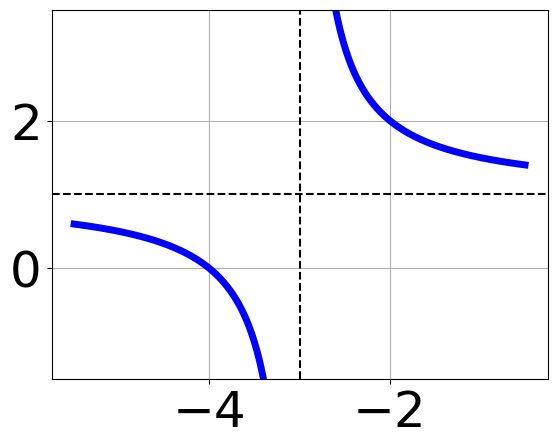
\includegraphics[width = 0.3\textwidth]{../Figures/rationalEquationToGraphCopyBC.png}\item 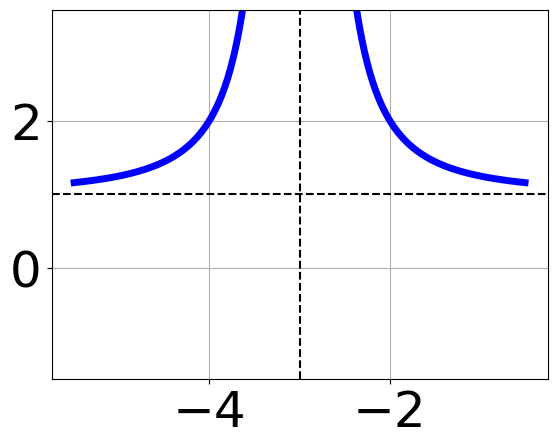
\includegraphics[width = 0.3\textwidth]{../Figures/rationalEquationToGraphCopyCC.png}\item 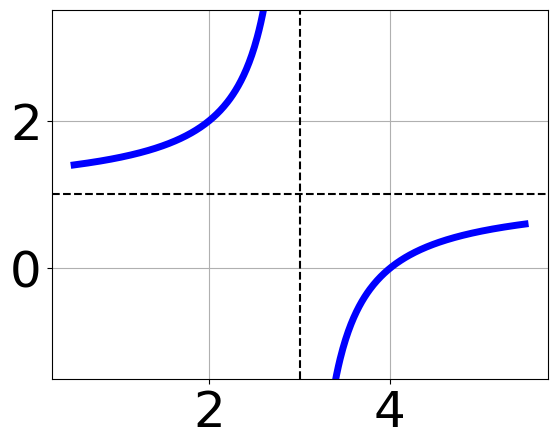
\includegraphics[width = 0.3\textwidth]{../Figures/rationalEquationToGraphCopyDC.png}\end{multicols}\item None of the above.
\end{enumerate} }
\litem{
Solve the rational equation below. Then, choose the interval(s) that the solution(s) belongs to.\[ \frac{7x}{-3x -5} + \frac{-4x^{2}}{-9x^{2} -36 x -35} = \frac{7}{3x + 7} \]\begin{enumerate}[label=\Alph*.]
\item \( x \in [-1.9,5] \)
\item \( x_1 \in [-4.3, -2.9] \text{ and } x_2 \in [-2.45,-0.81] \)
\item \( x \in [-3.2,-0.7] \)
\item \( x_1 \in [-4.3, -2.9] \text{ and } x_2 \in [-0.67,1.13] \)
\item \( \text{All solutions lead to invalid or complex values in the equation.} \)

\end{enumerate} }
\litem{
Choose the equation of the function graphed below.
\begin{center}
    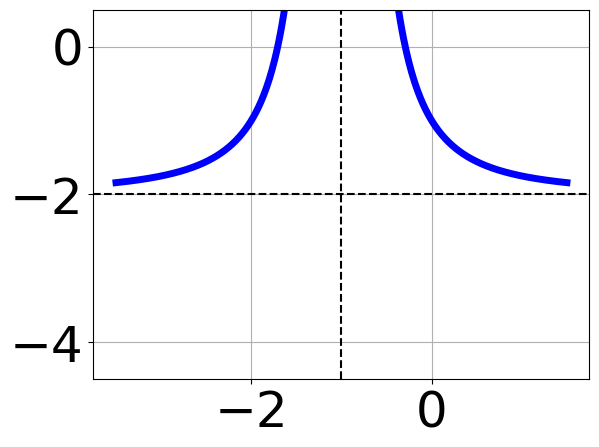
\includegraphics[width=0.5\textwidth]{../Figures/rationalGraphToEquationC.png}
\end{center}
\begin{enumerate}[label=\Alph*.]
\item \( f(x) = \frac{-1}{(x - 1)^2} - 2 \)
\item \( f(x) = \frac{-1}{x - 1} - 2 \)
\item \( f(x) = \frac{1}{x + 1} - 2 \)
\item \( f(x) = \frac{1}{(x + 1)^2} - 2 \)
\item \( \text{None of the above} \)

\end{enumerate} }
\litem{
Determine the domain of the function below.\[ f(x) = \frac{3}{12x^{2} -29 x + 15} \]\begin{enumerate}[label=\Alph*.]
\item \( \text{All Real numbers except } x = a, \text{ where } a \in [11.1, 14] \)
\item \( \text{All Real numbers except } x = a, \text{ where } a \in [-1.9, 1.2] \)
\item \( \text{All Real numbers except } x = a \text{ and } x = b, \text{ where } a \in [-1.9, 1.2] \text{ and } b \in [1.3, 3.6] \)
\item \( \text{All Real numbers.} \)
\item \( \text{All Real numbers except } x = a \text{ and } x = b, \text{ where } a \in [11.1, 14] \text{ and } b \in [12.8, 15.3] \)

\end{enumerate} }
\litem{
Choose the graph of the equation below.\[ f(x) = \frac{1}{(x + 2)^2} + 1 \]\begin{enumerate}[label=\Alph*.]
\begin{multicols}{2}\item 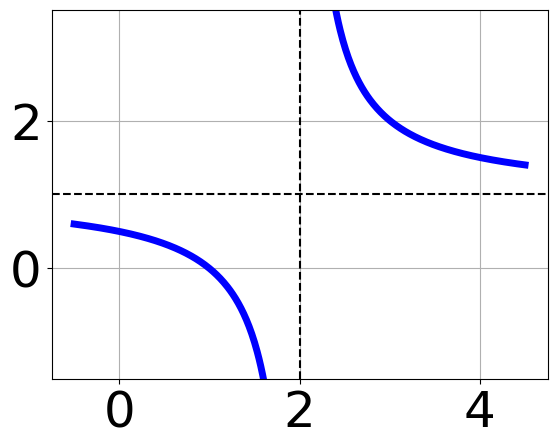
\includegraphics[width = 0.3\textwidth]{../Figures/rationalEquationToGraphAC.png}\item 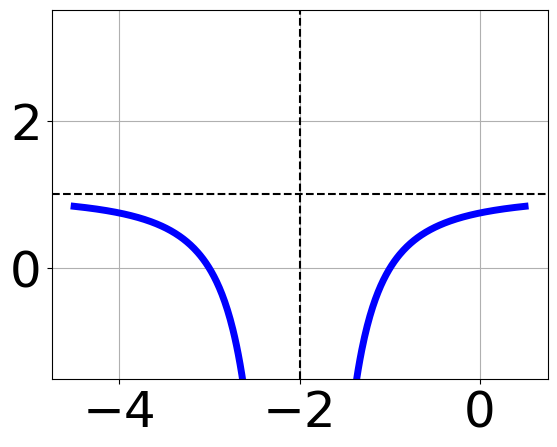
\includegraphics[width = 0.3\textwidth]{../Figures/rationalEquationToGraphBC.png}\item 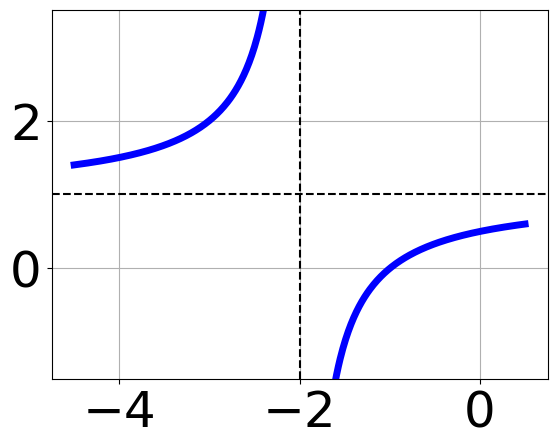
\includegraphics[width = 0.3\textwidth]{../Figures/rationalEquationToGraphCC.png}\item 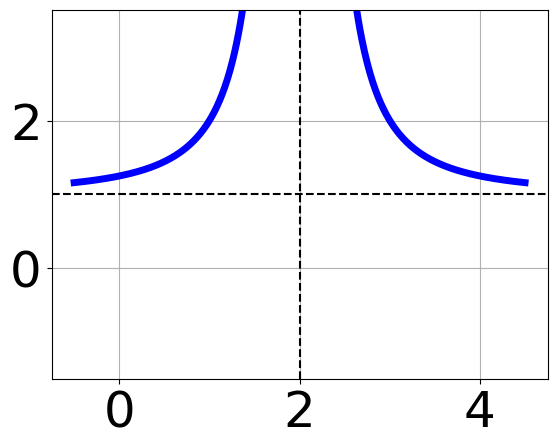
\includegraphics[width = 0.3\textwidth]{../Figures/rationalEquationToGraphDC.png}\end{multicols}\item None of the above.
\end{enumerate} }
\litem{
Solve the rational equation below. Then, choose the interval(s) that the solution(s) belongs to.\[ \frac{2x}{-7x -7} + \frac{-2x^{2}}{49x^{2} +98 x + 49} = \frac{-5}{-7x -7} \]\begin{enumerate}[label=\Alph*.]
\item \( x_1 \in [-2.08, -1.92] \text{ and } x_2 \in [-1.06,-0.56] \)
\item \( x \in [-1.07,-0.9] \)
\item \( x_1 \in [-2.08, -1.92] \text{ and } x_2 \in [-1.23,-1.13] \)
\item \( \text{All solutions lead to invalid or complex values in the equation.} \)
\item \( x \in [-1.4,-1.1] \)

\end{enumerate} }
\litem{
Solve the rational equation below. Then, choose the interval(s) that the solution(s) belongs to.\[ \frac{-4}{8x -6} + 9 = \frac{9}{64x -48} \]\begin{enumerate}[label=\Alph*.]
\item \( x \in [-0.18,1.82] \)
\item \( x_1 \in [-2.68, 0.32] \text{ and } x_2 \in [0.55,0.83] \)
\item \( x_1 \in [-0.18, 2.82] \text{ and } x_2 \in [0.84,1.26] \)
\item \( \text{All solutions lead to invalid or complex values in the equation.} \)
\item \( x \in [-2.68,0.32] \)

\end{enumerate} }
\end{enumerate}

\end{document}